% !TEX root = main.tex
\setcounter{chapter}{4}
\begin{lecture}[Много полезной хрени]
\section{Квантовый гармонический осциллятор}
Задается потенциалом
\begin{equation}
    \label{eq:harmonic_potential_def}
    V(x) = \frac{1}{2}\, m \omega^2 x^2
\end{equation}

Соотвествующее уравнение Шредингера:
\begin{equation}
    \label{eq:schrodinger_equation_harmonic}
    \left( -\frac{\hbar^2}{2m}\, \frac{d^2}{dx^2}\, + \frac{1}{2}\, m \omega^2 x^2 \right) \psi = E \psi
\end{equation}

Выбираем систему единиц с $\hbar = m = \omega = 1$ для простоты:
\begin{equation}
    \label{eq:schrodinger_equation_harmonic_atomic_units}
    \left( -\frac{1}{2}\, \frac{d^2}{dx^2}\, + \frac{1}{2}\, x^2 \right) \psi = E \psi
\end{equation}

Для уравнения \eqref{eq:schrodinger_equation_harmonic_atomic_units} существуют аналитические решения:
\begin{align}
    E_n &= n + \frac{1}{2} \\
    \psi &= \dots \text{эрмитовы функции} \dots
\end{align}

Важно заметить, что число волновой функции нулей равно номеру $n$ (из теории).
Это отображено на картинке \ref{fig:harmonic_levels}.

Все эти функции можно получить через программу \texttt{harmonic\_wavefunction.py} (листинг \ref{code:psi_harmonic_analytical}).
\begin{figure}[!h]
    \label{fig:harmonic_levels}
    \centering
    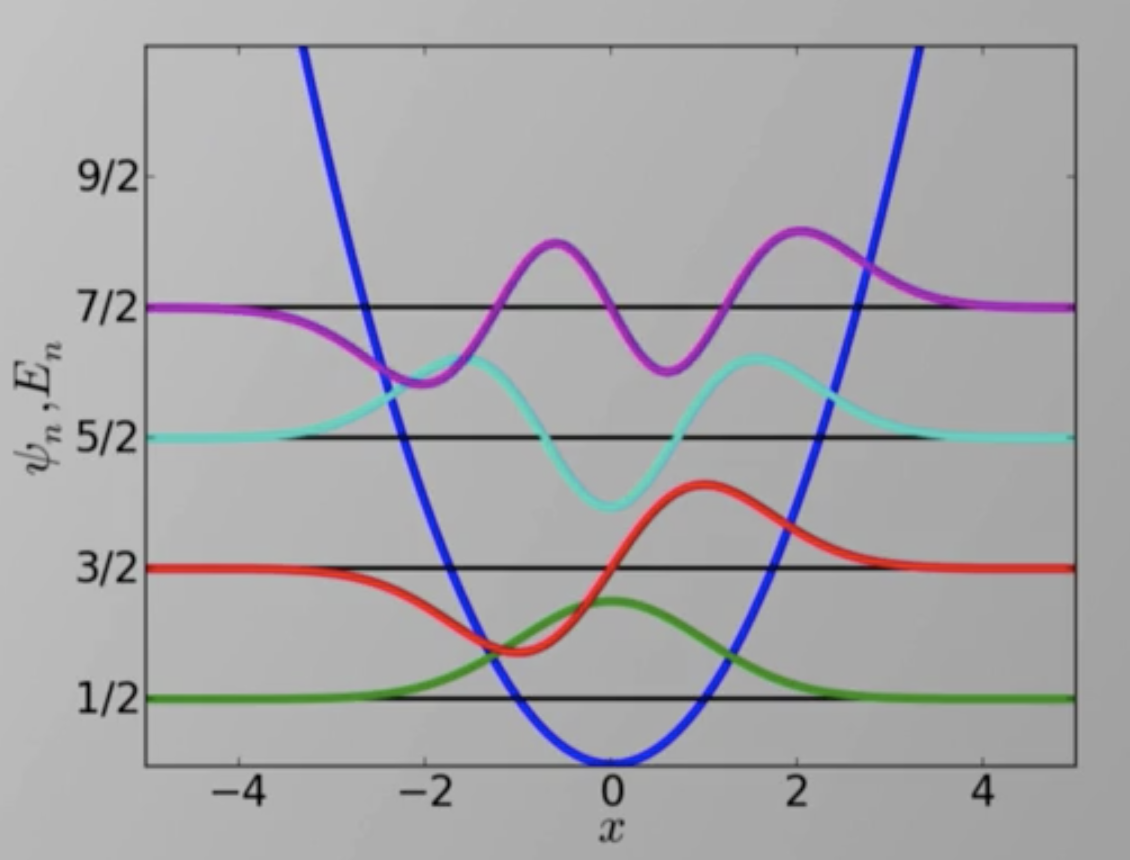
\includegraphics[width=0.6\textwidth]{harmonic_levels}
    \caption{Потенциал $V(x) = \frac{1}{2}\, x^2$, его уровни энергии и волновые функции.} 
\end{figure}
\newpage
\pythonfile{../w5/programs_lecture_5/harmonic_wavefunction}{Рекурсивная формула для подсчета $\psi (x)$ (\texttt{harminic\_wavefunction.py})}{code:psi_harmonic_analytical}

Основные свойства $\psi$:
\begin{itemize}
    \item Уход на ноль в бесконечностях: $\psi (x) \xrightarrow[x\rightarrow \pm \infty]{} 0$;
    \item Ортонормированность: $\int\limits_{- \infty}^{+\infty} dx \psi_n (x) \psi_m^* (x) = \delta_{mn}$;
\end{itemize}

В лекциях предлагают проверить, что результат программы \ref{code:psi_harmonic_analytical} действительно является решением УШ.
Для этого авторы предлагают насчитать $\cfrac{H \psi_{n}}{\psi_{n} }\, $ при разных $x$ и убедиться, что это примерно константа.
Сама программа для проверки приведена на листинге \ref{code:psi_harmonic_check}.

\pythonfile{../w5/programs_lecture_5/harmonic_wavefunction_check}{Проверка аналитической формулы для $\psi_\text{harmonic} (x)$}{code:psi_harmonic_check}

Обратите внимание, что в строке (19) используется дискретная аппроксимация второй производной (вычматы!).
\begin{figure}[!h]
    \label{fig:harmonic_check}
    \centering
    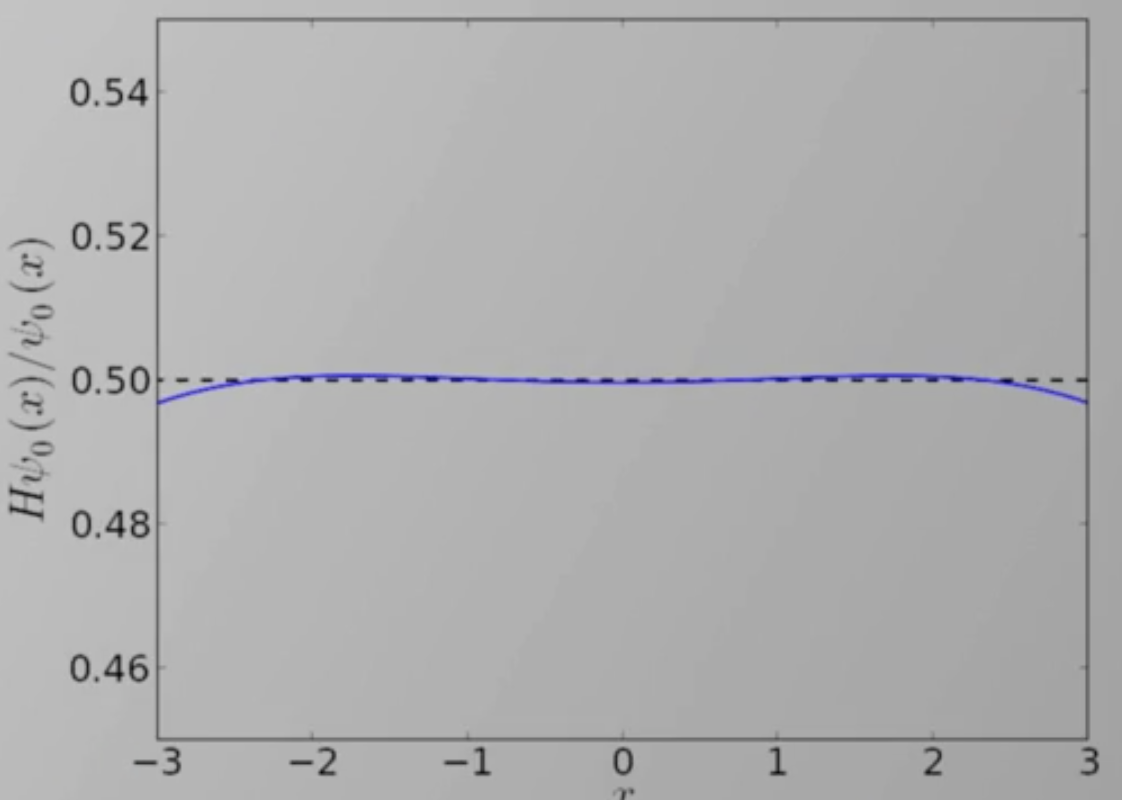
\includegraphics[width=0.6\textwidth]{harmonic_check}
    \caption{Численная проверка $H \psi_{n} / \psi_n$ при разных $x$}
\end{figure}

\section{Квантовая статистическая механика}
Два пункта, на которые стоит обратить внимание:
\begin{itemize}
    \item \textit{Квантовость} означает, что вероятность занять координату $x$ равна $|\psi (x)|^2$;
    \item \textit{Статистика} означает, что вероятность занять уровень $E_n$ идет по экспоненте: $\pi (n) \propto e^{-\frac{E_n}{k_B T}} $; 
\end{itemize}

Таким образом, мы имеем и распределение по уровням, и распределение по координатам внутри уровня.
Это записывается как $e^{-\beta E_n} |\psi_n (x)|^2$ --- \textit{вероятность быть в состоянии $n$ и координате $x$}.
\begin{equation}
    \label{eq:prob-E_n-coord_x}
    \pi (x, n) \propto \underbrace{e^{-\beta E_n}}_\text{Больцман} \underbrace{\psi_n (x) \psi_n^* (x)}_\text{Шредингер}
\end{equation}

Стоит заметить, что в \eqref{eq:prob-E_n-coord_x} встречаются два "мира": классический Больцман и квантовый Шредингер.
Тем не менее, ни уровни энергии $E_n$, ни волновые функции $\psi_n (x)$ не могут быть расчитаны, поэтому стоит искать другой подход.

\section{Матрица плотности: минимум}
Другой способ описания лежит через \textit{матрицу плотности} $\rho (x, x\prime, \beta)$.
О ней подробно рассказывается в Фейнмане \cite{feynman} (гл. 2 "Матрицы плотности"), откуда я любезно возьму большую часть материала.

В матрицах плотности рассматривается совокупность <<система + остальная Вселенная>>.
Пусть переменная $x$ описывает  координаты системы, а переменная $y$ --- координаты остальной части Вселенной. Пусть $\phi_i (x)$ представляет полный набор волновых функций. Тогда в наиболее общем виде любая волновая функция может быть записана в виде:
\begin{equation}
    \label{eq:psi-in-basis-phi-general}
    \psi (x, y) = \sum\limits_{i}^{} C_i (y) \phi_i (x).
\end{equation}
Перейдем к обозначениям Дирака. Пусть $\bra{\psi_i}$ есть полный набор векторов в векторном пространстве, описывающем систему, а $\bra{\theta_i}$ --- соответствующий набор для остальной части Вселенной:
\begin{align}
    & \phi_i (x) = \braket{x|\phi_i},
    & \theta_i (y) = \braket{y|\theta_i}
\end{align}
Тогда ВФ записывается как:
\begin{align}
    \label{eq:psi-in-basis-phi-theta-general}
    & \ket{\psi} = \sum^{}_{ij} C_{ij} \ket{\phi_i} \ket{\theta_j} \\
    & \psi (x, y) = \bra{y}\braket{x|\psi} = \sum^{}_{ij} C_{ij} \braket{x|\phi_i} \braket{y|\theta_j}
\end{align}
Выражение \eqref{eq:psi-in-basis-phi-general} получается, если положить:
\begin{equation}
    \label{eq:C_i-basis-definition}
    C_i (y) = \sum\limits_{i}^{} C_{ij} \braket{y|\theta_j}
\end{equation}

Пусть оператор $A$ действует только на систему.
Тогда он определяется выражением (в базисе $\ket{\phi_i}\ket{\theta_i}$):
\begin{equation}
    \label{eq:A-action-on-system-general}
    \sum\limits_{ii'j}^{} A_{ii'} \ket{\phi_i} \ket{\theta_j} \bra{\theta_j} \bra{\phi_{i'}}.
\end{equation}
По сути, здесь мы впихнули теорфизовское определение единицы: $\sum\limits_{i}^{} \ket{\theta_i} \bra{\theta_i} = 1$.

Теперь можно подсчитать среднее значение $A$:
\begin{align}
    \label{eq:A-mean-derivation}
    \nonumber
    & \braket{A} =
    \braket{\psi|A|\psi} =
    \underbrace{\sum\limits_{ij}^{} C_{ij}^* \bra{\phi_i}\bra{\theta_j}}_{\bra{\psi}}
    A
    \underbrace{\sum\limits_{i'j'}^{} C_{i'j'} \ket{\phi_{i'}} \ket{\theta_{j'}}}_{\ket{\psi}} = \\
    & \sum\limits_{ij, i'j'}^{} C_{ij}^{*} C_{i'j'} \bra{\theta_j} \braket{\phi_i|A|\phi_{i'}} \ket{\theta_{i'} } =
    \sum_{iji'}^{} C_{ij}^* C_{i'j'} \braket{\phi_i|A|\phi_{i'} } =
    \sum\limits_{ii'}^{} \braket{\phi_i|A|\phi_{i'} }    \rho_{i'i}
\end{align}
где введена матрица плотности:
\begin{equation}
    \label{eq:rho-definition-from-C}
    \rho_{i'i} = \sum\limits_{j}^{} C_{ij} ^{*} C_{i'j}
\end{equation}

Поразмышляем над этим определением.
Здесь идет суммирование по $j$ -- а этот индекс соответствовал $\ket{\theta_j}$ в разложении по базису.
Получается, что мы как бы делаем свертку вдоль всевозможных состояний Вселенной двух состояний: $i$-ого и $i'$-ого состояний самой подсистемы.
Более того, $\rho_{ii}$ соответствует амплитуде вероятности занять $i$-ое состояние, поэтому $\rho_{i'i}$ похоже на <<кореллированность>> состояний $i'$ и $i$.

Осталось чуть-чуть.
Введем оператор $\hat{\rho}$ таким образом: $\rho_{i'i} = \braket{\phi_{i'}| \hat{\rho} | \phi_i}$, причем $\hat{\rho}$ действует только на переменные $x$.
Тогда
\begin{equation}
    \braket{\phi|A|\psi} = \braket{A} =
    \sum\limits_{ii'}^{} \braket{\phi_i|A|\phi_{i'} }    {\color{red} \rho_{i'i}} =
    \sum\limits_{i}^{} \bra{\phi_i} A 
    \underbrace{\sum\limits_{i'} \ket{\phi_{i'}} \bra{\phi_{i'}}}_{=1}
    \hat\rho \ket{\phi_i} =
    \sum\limits_{i}^{} \braket{\phi_i | A \hat{\rho} | \phi_i} = \Sp \hat{\rho} A
\end{equation}

Из \eqref{eq:rho-definition-from-C} видно, что $\hat{\rho} $ --- эрмитов оператор.
Его тогда можно диагонализовать и собственные значения $w_i$ действительны, а собственные векторы $\ket{i}$ образуют полный ортонормированный набор:
\begin{equation}
    \label{eq:rho-in-own-basis}
    \rho = \sum\limits_{i}^{} w_i \ket{i} \bra{i}.
\end{equation}

Можно показать, что $w_i \geq 1$ и $\sum\limits_{i}^{} w_i = 1$.

\section{Уход от волновых функций к матрице плотности}

Теперь \textit{важный} переход: мы можем уйти от волновых функций и целиком описывать систему через $\rho$.
Для этого надо ввести следующие положения:
\begin{enumerate}
    \item векторы $\ket{i}$ образуют полный ортонормированный базис;
    \item $w_i \geq 0$;
    \item $\sum\limits_{i}^{} w_i = 1$;
    \item среднее значение оператора $A$ определяется как $\braket{A} = \Sp \hat{\rho} A$.
\end{enumerate}

В этом формализме можно получить $\hat{\rho} (t)$.
Переписывая \eqref{eq:rho-in-own-basis} в виде
\begin{equation}
    \label{eq:rho-in-own-basis-time}
    \rho (t) = \sum\limits_{i}^{} w_i \ket{i(t)} \bra{i (t)}
\end{equation}
можно разложить состояние $\ket{i(0)}$ по собственным функциям гамильтониана $H$, а изменение последних известно (оператор эволюции в помощь).
Тогда можно сразу сказать, что
\begin{equation}
    \label{eq:i-th_state_time_evolution}
    \ket{i(t)} = e^{-i \hat{H}t} \ket{i(0)}.
\end{equation}
и для оператора $\hat{\rho}$:
\begin{align}
    \label{eq:rho-time-evolution}
    & \rho (t) = e^{-i \hat{H} t} \rho (0) e^{i \hat{H}t},
    & \dot \rho = -i (H\rho - \rho H)
\end{align}

Запись матрицы плотности в координатном представлении имеет вид:
\begin{equation}
    \rho (x, x') = \int\limits_{}^{} \psi (x, y) \psi^* (x', y) dy
\end{equation}
который легко получить, если смотреть на $C_i \rightarrow C_x$ как на коэффициенты разложения в координатном представлении: $\hat{x} \ket{x} = C_x \ket{x}$ и считать, что функция $\psi (x) = \braket{x|\psi} = \bra{x}\sum\limits_{x'}^{} C_{x'}\ket{x'} = \delta_{xx'} C_{x'} = C_x$.

\section{Матрицы плотности в моделировании}
Запись \eqref{eq:prob-E_n-coord_x} можно свести к матрицам плотности:
\begin{equation}
    \label{eq:rho-via-E_n-coord_x}
    \rho (x, x', \beta) = \sum\limits_{n}^{} e^{-\beta E_n} \psi_n (x) \psi_n^* (x')
\end{equation}

Это дает кучу плюшек. Например, можно подсчитать статсумму:

\begin{equation}
    \label{eq:Z-rho-is-correct}
    \begin{aligned} 
        Z(\beta) &=\operatorname{Tr} \rho=\int_{-\infty}^{+\infty} d x \rho(x, x, \beta) =\int_{-\infty}^{+\infty} d x \sum_{n} e^{-\beta E_{n}} \psi_{n}(x) \psi_{n}^{*}(x) \\ &=\sum_{n} e^{-\beta E_{n}} \int_{-\infty}^{+\infty} d x \psi_{n}(x) \psi_{n}^{*}(x) = \sum_{n} e^{-\beta E_{n}} 
    \end{aligned}
\end{equation}

Но самое главное, что можно подчерпнуть из \eqref{eq:prob-E_n-coord_x-via-rho} --- это \textit{свойство конволюции}.
\subsection{Свойство конволюции}
\begin{align}
    \label{eq:rho_convolution-derivation}
    \nonumber
    & \boxed{\int\limits_{}^{} dx' {\color{red}\rho(x, x', \beta_1)} {\color{blue}\rho(x', x'', \beta_2)}} =
    \int d x^{\prime} \sum_{{\color{red}n}, {\color{blue}m}} 
    {\color{red}\psi_{n}(x) e^{-\beta_{1} E_{n}} \psi_{n}^{*}\left(x^{\prime}\right)} 
    {\color{blue} \psi_{m}\left(x^{\prime}\right) e^{-\beta_{2} E_{m}} \psi_{m}^{*}\left(x^{\prime \prime}\right)} = \\
    & = \sum_{n, m} \psi_{n}(x) e^{-\beta_{1} E_{n}} \underbrace{\int d x^{\prime} \psi_{n}^{*}\left(x^{\prime}\right) \psi_{m}\left(x^{\prime}\right)}_{\delta_{n m}, \text { orthogonality }} e^{-\beta_{2} E_{m}} \psi_{m}^{*}\left(x^{\prime \prime}\right) = \sum_{n} \psi_{n}(x) e^{-\left(\beta_{1}+\beta_{2}\right) E_{n}} \psi_{n}^{*}\left(x^{\prime \prime}\right) =
    \boxed{\rho\left(x, x^{\prime \prime}, \beta_{1}+\beta_{2}\right)}
\end{align}

В частности,
\begin{equation}
    \label{eq:rho_convolution-2beta}
    \int\limits_{}^{} dx' \underbrace{\rho(x, x', \beta) \rho(x', x'', \beta)}_\text{high temperature} =
    \underbrace{\rho (x, x'', 2\beta)}_\text{low temperature}
\end{equation}

\subsection{Матрица плотности свободной частицы}
Для свободной частицы матрицу плотности можно найти аналитически (см. вывод в \cite{feynman}).
Там получается из \eqref{eq:rho-time-evolution} уравнение диффузии, которое сразу решается (с учетом нормировки):
\begin{equation}
    \label{eq:rho-free-particle}
    \rho^\text{free} (x, x', \beta) = \frac{1}{\sqrt{2\pi \beta}}\, \exp \left( -\frac{(x - x')^2}{2\beta}\, \right)  
\end{equation}

\subsection{Trotter decomposition}
Для гамильтониана $\hat{H} = \hat{H}^{\text{free}} + V(x)$ при $\beta \rightarrow 0$ (\textbf{высокие температуры}) выполнено:
\begin{equation}
    \label{eq:trotter-decomposition-definition}
    \rho (x, x', \beta) = e^{- \frac{\beta}{2}\, V(x)} \rho^{\text{free}} (x, x', \beta) e^{- \frac{\beta}{2}\, V(x')} 
\end{equation}

В листинге \ref{code:matrix_square_harmonic} можно увидеть, как меняется от этого heatmap для $\rho (x, x', \beta)$.

\pythonfile{../w5/programs_lecture_5/matrix_square_harmonic}{Программа для подсчета $\rho$ в приближении Trotter decomposition}{code:matrix_square_harmonic}

\section{Path integral и метод Монте-Карло}
Вычислять $\rho$ через \eqref{eq:rho-via-E_n-coord_x} очень затратно, поскольку почти невозможно удержать в памяти все $E_n$ и дискретную аппроксимацию $\psi (x)$.
Но у нас есть ведь свойство конволюции \eqref{eq:rho_convolution-2beta}!
Возникает идея продолжать процесс \eqref{eq:rho_convolution-2beta} до допустимого предела, а затем подставить $\rho^{\text{free}} $ при высоких температурах.

Это вполне здравая мысль, но взятие кратных интегралов может стать проблемой.
Более того, в пределе, когда разбиение продолжается бесконечно, мы приходим к т.н. \textit{континуальному интегралу}.
Основной способ бороться с ними --- свести к Path Integral (см. \cite{feynman}).

Пользуясь свойством конволюции в общем виде \eqref{eq:rho_convolution-derivation}, получим:
\begin{equation}
    \label{eq:rho_convolution_N-times}
    \rho (x_0, x_N, \beta) =
    \int d x_{1} d x_{2} \ldots d x_{N-1} \rho\left(x_{0}, {\color{red}x_{1}}, \beta / N\right) \rho\left({\color{red} x_{1}}, x_{2}, \beta / N\right) \ldots \rho\left(x_{N-1}, x_{N}, \beta / N\right)
\end{equation}
Логика проста: второй аргумент сцепливается с первым у следующего множителя и т.д.
Как бы было ранее, $Z (\beta)$ есть просто
\begin{equation}
    \label{eq:Z_N-times_convolution}
    Z (\beta) = \int dx_0 \rho (x_0, x_0, \beta) =
    \int {\color{red} d x_{0}} d x_{1} \ldots d x_{N-1} \rho\left({\color{red} x_{0}}, x_{1}, \beta / N\right) \rho\left(x_{1}, x_{2}, \beta / N\right) \ldots \rho\left(x_{N-1}, {\color{red} x_{0}}, \beta / N\right)
\end{equation}

Теперь мы готовы обсуждать Path Integral.

\subsection{Path Integral}
Поскольку в дальнейшем вычисления будут проводиться на компьютере, имеет смысл рассмотреть дискретную аппроксимацию \eqref{eq:Z_N-times_convolution}. При этом будем считать, что интеграл в выражении \eqref{eq:Z_N-times_convolution} сходится.

Из сходимости интеграла следует, что в дискретной аппроксимации мы можем брать произвольное разбиение на жордановы множества (в данном случае мы будем брать \textit{только} клетки) и произвольную выборку точек --- лишь бы мелкость разбиения стремилась к нулю.

Если множество интегрирования (многомерный куб) разбить на множество кубиков одинакового объема $\Delta V$ (их будет $M^N$ штук), а вдоль каждой оси $x_i$ сделать выборку из $M$ точек, то в дискретной аппроксимации \eqref{eq:Z_N-times_convolution} перепишется в виде:
\begin{align}
    \label{eq:Z_N_times_convolution-discrete}
    & Z (\beta) \approx \sum\limits_{x_0 \in \{x_0^{(1)}, \dots, x_0^{(M)}\}} \dots \sum\limits_{x_{N-1} \in \{x_{N-1}^{(1)}, \dots, x_{N-1}^{(M)}\}}
    \rho (x_0, {\color{red} x_1}, \beta / N) \cdot \rho ({\color{red} x_1}, x_2, \beta / N) \cdot \dots \\
    & \ldots \cdot \rho (x_{N-2}, {\color{red} x_{N-1}}, \beta / N) \cdot \rho ({\color{red} x_{N-1}}, x_0, \beta / N) \Delta V
\end{align}

Будем считать функцию $\rho (x, x', \beta)$ нормированной по $x$, $x'$: $\int dx dx' \rho (x, x', \beta) = 1$.
Если это не так, то всегда функцию можно поделить на этот интеграл (предполагая, что он конечный) и тем самым нормировать.
Для получения $Z(\beta)$ останется только в конце домножить на поделенное значение.

В этом случае на функцию $\rho (x_i, x_{i+1}, \beta / N)$ в \eqref{eq:Z_N_times_convolution-discrete} можно смотреть как на функцию вероятности перехода из $x_i$ в $x_{i+1}$ в некотором марковском процессе. 
Тогда произведение внутри суммы $\rho (x_0, x_1, \beta /N)\cdot~\dots~\cdot\rho(x_{N-1}, x_0, \beta /N)$ есть вероятность пройти путь из $x_0$ в $x_0$, проходя при этом через промежуточные точки $x_1, x_2, \dots, x_{N-1} $, т.е. вероятность осуществить \textit{путь} $x_0 \rightarrow x_1 \rightarrow \dots \rightarrow x_{N-1} \rightarrow x_0$. 


% \begin{wrapfigure}{r}{0.2\textwidth}
%     \label{fig:path-integral-schema}
%     \centering
%     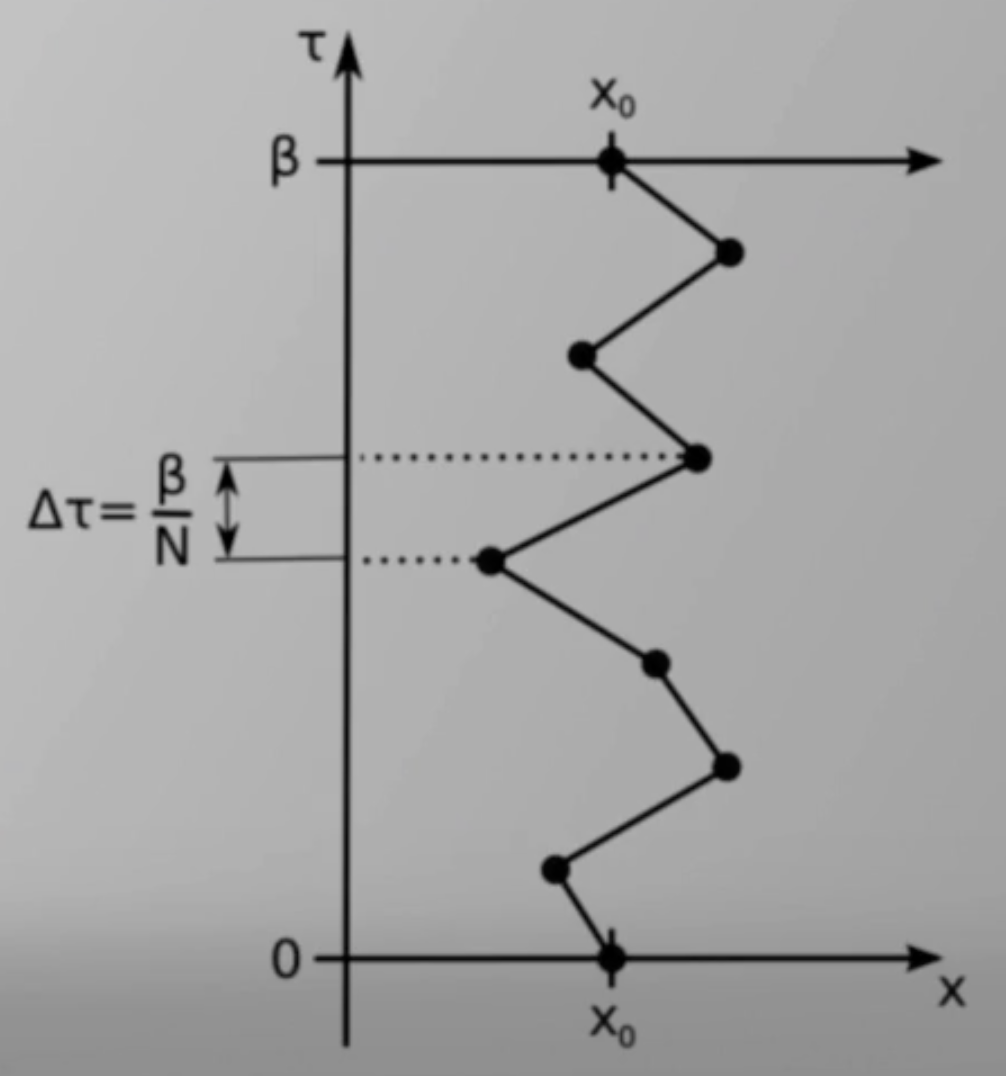
\includegraphics[width=0.2\textwidth]{path-integral}
%     \caption{Иллюстрации пути в Path Integral}
% \end{wrapfigure}
Какую же тогда роль играет $\beta /N$?
Посмотрим еще раз на произведение. Каждый из множителей как бы <<собирает>> $\beta /N$ до конечного состояния $\beta = N \cdot \beta /N$.
Например, первые два множителя дадут своим вкладом $2\beta /N$, три множителя --- $3\beta /N$ и так далее.
Этому свойству <<аккумулирования шаг за шагом>> удовлетворяет в марковских процессах \textit{время} : оно тоже за каждый дискретный шаг увеличивается на некоторую величину $\Delta \tau$.
Можно тогда сказать, что $\beta /N$ является своего рода временем (в курсе его называют \textit{мнимым временем}), а сам процесс --- марковским переходом из $x_0$ в $x_0$ через $x_1, \dots, x_{N-1} $ с дискретным шагом времени $\Delta \tau = \beta /N$.
Это можно изобразить на рисунке:
\end{lecture}
